\section{Proprietà dei Nuclei}
Lo studio dei nuclei è essenziale per molte applicazioni e ci porterà a comprendere i motivi di alcuni effetti che si generano, come per esempio il motivo del decadimento $\beta$. 
Questa sezione sarà quindi essenziale per la comprensione di molti effetti che verranno descritti poi.
%nuova sezione--------------------------------------------------
\subsection{Spin Nucleare e Momento Magnetico}
Molte proprietà dei nuclei si caratterizzano in modo fenomenologico, ovvero per analogia con effetti già conosciuti.
Lo spin viene descritto in analogia a ciò che viene studiato in struttura della materia e meccanica quantistica. 
Ricordiamo ora com'è caratterizzato il moto dell'elettrone attorno al nucleo, questo si descrive come un moto di rivoluzione e di rotazione.
\begin{figure}[h]
\centering
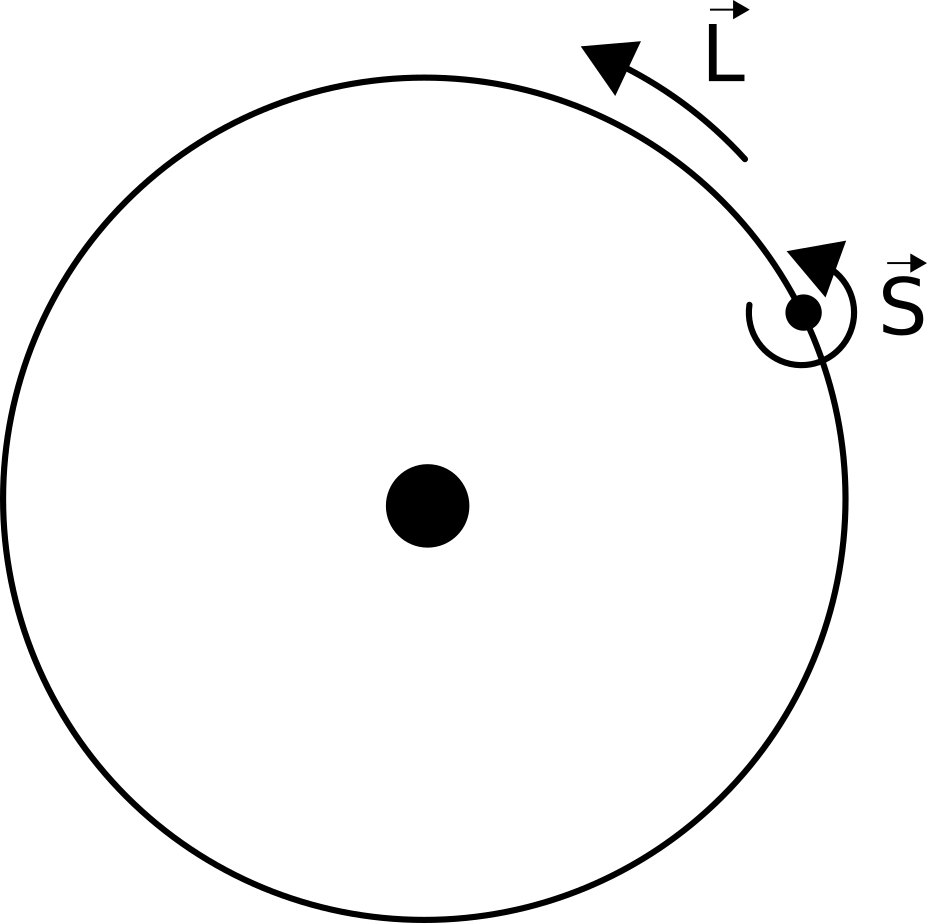
\includegraphics[width=150pt]{fig3_01}
\end{figure}
Vi sono inoltre più numeri quantici che caratterizzano l'elettrone:
\begin{equation}
\begin{split}
n\hspace{1cm} & 1, 2,3\\
L\hspace{1cm} & 0\to N-1\\
m\hspace{1cm} & -L\to0\to+L\\
s\hspace{1cm} & +\frac{1}{2}, -\frac{1}{2}
\end{split}
\end{equation}
Per quanto riguarda i nucleoni, il fatto di avere un momento angolare non è banale, non vi è infatti un potenziale centrale che ne giustifichi la presenza.
La questione è valida in quanto dimostrata da fatti sperimentali.
Per ogni nucleone, all'interno del nucleo, possiamo definire un momento angolare totale che è dato da 
\begin{equation}
\bar s =\bar l + \bar s
\end{equation}
e con lo stesso tipo di analogia potremo trovare quello che si chiama spin del nucleo, ottenuto come la somma di tutti gli spin dei nucleoni.
\begin{equation}
I=\sum \bar s
\end{equation}
La spiegazione deriva dal fatto che siccome i protoni sono particelle cariche, e una particella carica in moto genera un momento magnetico, si otterrà anche per i nucleoni un momento magnetico.

\paragraph{un paio di commenti}
\begin{itemize}
\item L'analogia dello spin di una particella con una trottola è una assunzione ben posta?
Si parte dal raggio classico dell'elettrone, ovvero il raggio che una carica avrebbe se tutta la sua massa fosse costituita da energia elettrostatica.
\begin{equation}
\begin{split}
m_e c^2=\frac{1}{4\pi\varepsilon_0}\frac{e^2}{r_e}\hspace{0.2cm}\to\hspace{0.2cm}r_e & =\frac{1}{4\pi\varepsilon_0}\frac{e^2}{m_ec^2}=\\
&=\frac{e^2\hbar c}{4\pi \varepsilon_0\hbar c}\frac{1}{m_ec^2}=\\
&=1,44MeV\cdot fm\frac{1}{0,5MeV}\sim 3fm
\end{split}
\end{equation}
In realtà noi consideriamo l'elettrone come una particella priva di struttura il che ci fa capire quanto sbagliata sia la nostra concezione di questi fenomeni. 
Il raggio reale è approssimabile a $0$.
Supponiamo che il momento angolare dell'elettrone sia \emph{(consideriamo qui l'elettrone come una sferetta con tutta la massa concentrata al bordo della sfera)}:
\begin{equation}
\hbar=r_e m_e v_e
\end{equation}
Qual è la velocità di questa sfera (elettrone)?
\begin{equation}
\begin{split}
v_e&=\frac{\hbar}{r_em_e}\to\frac{v_e}{c}\\
&=\frac{\hbar c}{r_em_e^2}\sim 10^2
\end{split}
\end{equation}

Il risultato ottenuto è assurdo, perché viola le regole base della relatività. 
L'analogia con la trottola è quindi un espediente utile alla comprensione ma errato e lo spin è da considerarsi un effetto puramente relativistico.
\item Qual è il cammino libero medio del nucleone nel nucleo?
Si ha
\begin{equation}
l=\frac{1}{n\delta}
\end{equation}
dove $\delta_{n-n}\sim 22MeV=300 mb$ è la sezione d'urto d'interazione e $n$ è alla densità numerica dei nucleoni nel nucleo.
\begin{equation}
n=\frac{A}{V}=\frac{A}{\frac{4}{3}\pi R_0^3 A}=\frac{3}{4(3,14)(1,15fm)^3}=0,16\frac{nucleoni}{fm^3}
\end{equation}
Il libero cammino medio sarà quindi
\begin{equation}
l=\frac{1}{0,16fm^3}\frac{1}{300\times 10^{-3}\cdot10^{-28}m^2\cdot 10^{30}fm^2/m^2}=0,21fm
\end{equation}
Il libero cammino medio corrisponde quindi a meno della dimensione del nucleone stesso, il che non fa ben sperare alla possibilità di spostamento dei nucleoni e alla conseguente esistenza di un momento magnetico.
In realtà c'è possibilità di movimento grazie al principio di esclusione di Pauli.
\end{itemize}

Dal punto di vista sperimentale quello che noi vediamo è che i nuclei hanno un certo momento magnetico (rather than l'effetto del momento angolare).
\begin{figure}[h]
\centering
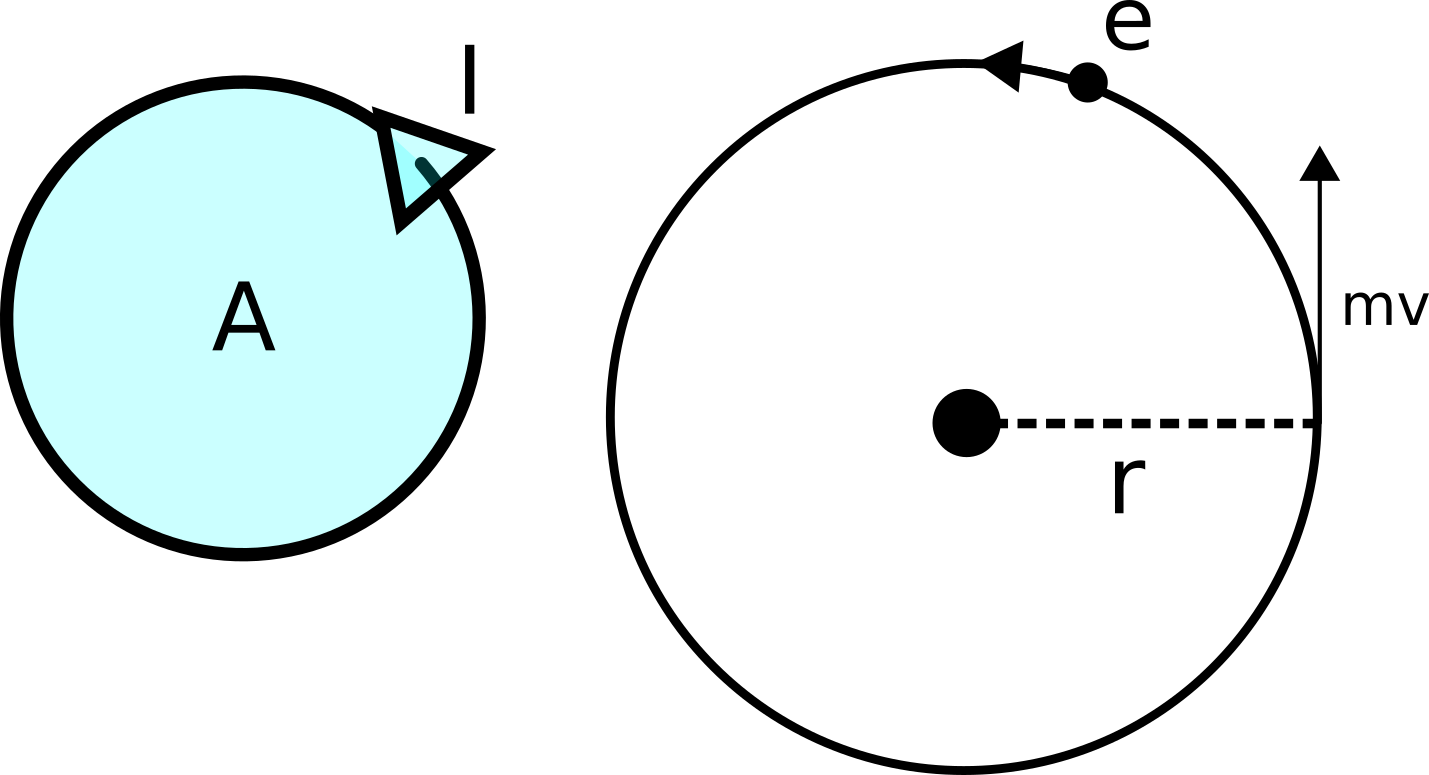
\includegraphics[width=200pt]{fig3_02}
\end{figure}
Il momento magnetico associato ad una carica in moto classicamente corrisponde alla corrente che attraversa una spira per l'area della spira stessa.
\begin{equation}
\mu=IA
\end{equation}

Prendendo ora il caso dell'elettrone (che poi sarà ampliato per analogia al caso dei nucleoni) si ha 
\begin{equation}
L=mvr, \hspace{0.5cm}I=\frac{e}{v}
\end{equation}
\begin{equation}
v=\frac{2\pi r}{t}\to t=\frac{2\pi r}{v}
\end{equation}
Si ottiene così la corrente generata da un elettrone
\begin{equation}
I=\frac{e}{2\pi r}v
\end{equation}
il che può essere sostituito nel momento magnetico per ottenere
\begin{equation}
\mu=IA=\frac{e}{2\pi r}v\pi r^2=\frac{evr}{2}\frac{mvr}{mvr}=\frac{e}{2m}L
\end{equation}
Il \emph{momento magnetico} di una particella carica è quindi
\begin{equation}
\mu=\frac{e}{2m}L
\label{PN:02}
\end{equation}
Dove la quantità $e/2m$ viene definita come \emph{rapporto giromagnetico}. 
Il momento ~\eqref{PN:02} fa riferimento alla meccanica classica ma può essere validato per la meccanica quantistica effettuando la sostituzione del momento angolare con $\hbar$.
Si ottiene così il \emph{magnetone di Bohr}
\begin{equation}
\mu_B=\frac{e}{2m_e}\hbar
\end{equation}
Questa è l'unità fondamentale per quanto riguarda il momento magnetico.
Possiamo poi ampliare questa definizione trovando il momento di dipolo magnetico dell'elettrone
\begin{equation}
\mu_e =\mu_B \frac{L}{\hbar}
\label{PN:01}
\end{equation}
Si può ora introdurre il fattore giromagnetico $g$ che ci permette di generalizzare la formula ~\eqref{PN:01}
\begin{equation}
\mu_B =g\mu_B \frac{L}{\hbar}
\end{equation}
A questi livelli di grandezza non si ha la certezza che carica e massa coincidano, anzi potrebbero essere totalmente indipendenti; questo fattore assume che ci sia una relazione ben definita tra momento angolare e momento magnetico, in particolare se distribuzione di massa e di carica coincidono $g=1$.
La trattazione ha comunque dei limiti, infatti quando verrà studiato lo \emph{spin} del nucleo si potrà notare come massa e carica non coincidano, ma per ora va bene che ci siano dei limiti nel calcolo.
Nel caso dell'elettrone che gira attorno al nucleo è vero che $g=1$.

Nel caso dei nucleoni all'interno del nucleo si ha per il protone:
\begin{equation}
\mu_p=\mu_N\frac{L}{\hbar}\hspace{1cm}\mu_N=\frac{e\hbar}{2m_p}
\end{equation}
dove $g=1$ e $\mu_N$ è detto magnetone nucleare.
Mentre per il neutrone:
\begin{equation}
\mu_n=0
\end{equation}

Per quanto riguarda lo \emph{spin} si ha che la relazione diventa
\begin{equation}
\mu_e=g\mu_B \frac{S}{\hbar}
\end{equation}
In questo il momento giromagnetico non sarà più $1$ ma si avrà $g_e=2$.
Questo valore si ottiene dall'equazione di Dirac per particelle prive di struttura interna.
Dall'elettrodinamica quantistica si ottiene poi che in realtà non è propriamente 2 ma $g=2,0023$ che coincide con una piccola variazione ma che deriva da cambiamenti importanti (tanto da essere scritta sull'epitaffio dello scopritore).
Nel caso dei nucleoni si ha
\begin{equation}
\mu_{p,n}=g_{p,n}\mu_N\frac{S}{\hbar}
\end{equation}
dove i fattori g corrispondono a $g_p=5,585691; g_n=-3,826084$.
Il fatto che questi fattori siano diversi da 2 ci fa capire come i nucleoni abbiano entrambi una struttura interna; si ha inoltre che il $g\not0$ per il neutrone implica che pure quest'ultimo possieda un momento magnetico pur essendo privo di carica.

Il momento di dipolo magnetico totale del nucleo è
\begin{equation}
\mu_N=\sum_p \left(\mu_N \frac{\bar{L}}{\hbar}+g_p\mu_N\frac{\bar S}{\hbar}\right)+\sum_n \biggl[g_n \mu_N\frac{\bar S}{\hbar}\biggl]
\end{equation}
\begin{figure}[h]
\centering
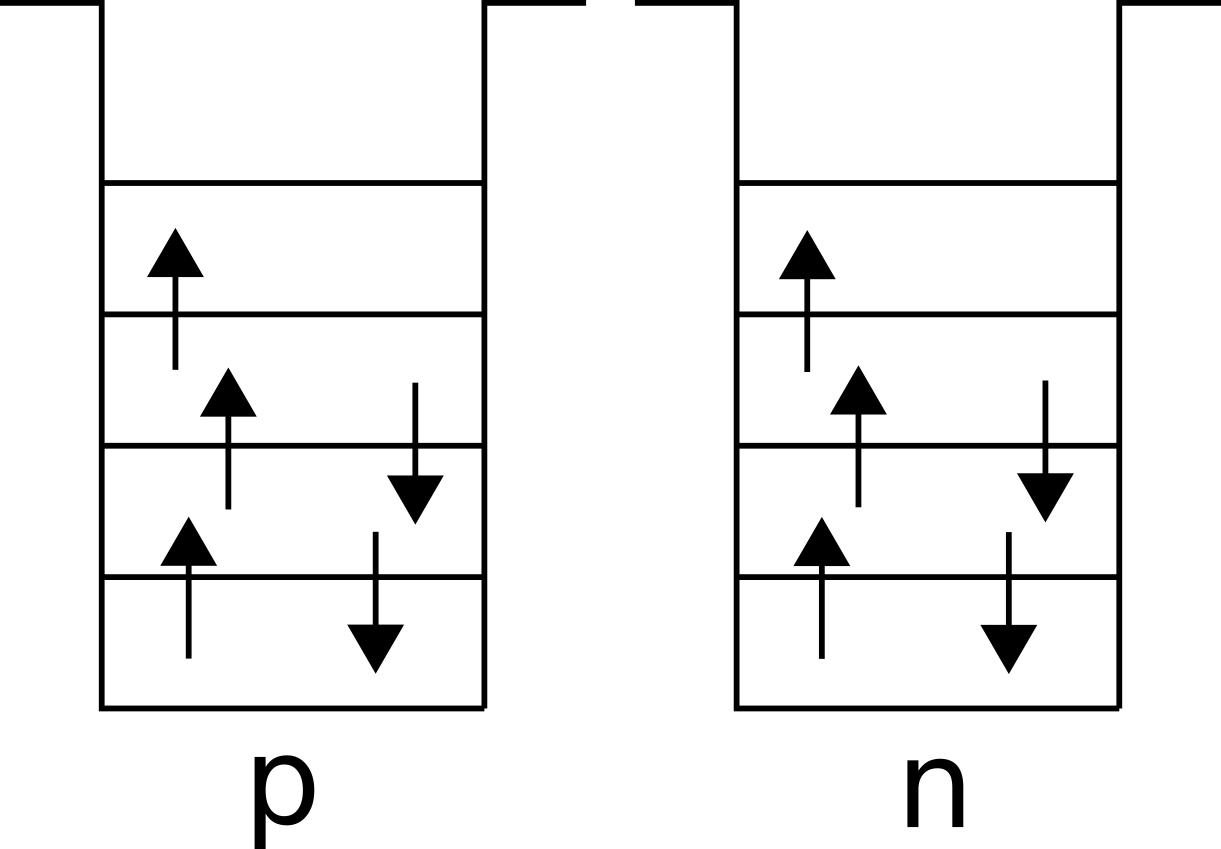
\includegraphics[width=180pt]{fig3_03}
\caption{Rappresentazione delle buche di potenziale dei protoni e dei neutroni}
\end{figure}
Una cosa interessante riguardo i neutroni e i protoni è che queste particelle sono fermioni ovvero particelle che soddisfano alla statistica di Fermi-Dirac (non posso avere più di una particella nello stesso stato, posso avere al massimo due particelle alla stessa energia con spin antiparallelo).
Essendo poi particelle all'interno di una buca di potenziale si può già intuire quale sarà lo spin del nucleo.
Per esempio:
\begin{itemize}
\item se il numero di massa A è pari e il numero atomico Z è dispari, avremo un numero dispari di neutroni e di protoni, in questo caso il nucleone spaiato (sia dalla parte dei neutroni che dei protoni) mi fa dire che avremo un nucleo con spin intero.
\item Se invece il numero totale di nucleoni è pari e il numero di protoni e neutroni è pari si avrà spin del nucleo nullo.
\item Se il numero di massa sarà dispari sappiamo che lo spin del nucleo è semi-intero.
\end{itemize} 